%% Copyright 2007-2026 Elsevier Ltd
%% This file is part of the 'Elsarticle Bundle'.
%% ---------------------------------------------
%% It may be distributed under the conditions of the LaTeX Project Public
%% License, either version 1.3 of this license or (at your option) any
%% later version.  The latest version of this license is in
%%    http://www.latex-project.org/lppl.txt
%% and version 1.3 or later is part of all distributions of LaTeX
%% version 1999/12/01 or later.
%% 
%% The list of all files belonging to the 'Elsarticle Bundle' is
%% given in the file `manifest.txt'.
%% 
%% Template article for Elsevier's document class `elsarticle'
%% with numbered style bibliographic references
%% SP 2008/03/01
%% $Id: elsarticle-template-num.tex 289 2026-01-09 06:13:01Z rishi $
%%
\documentclass[review,12pt]{elsarticle}

%% Use the option review to obtain double line spacing
%% \documentclass[authoryear,preprint,review,12pt]{elsarticle}

%% Use the options 1p,twocolumn; 3p; 3p,twocolumn; 5p; or 5p,twocolumn
%% for a journal layout:
%% \documentclass[final,1p,times]{elsarticle}
%% \documentclass[final,1p,times,twocolumn]{elsarticle}
%% \documentclass[final,3p,times]{elsarticle}
%% \documentclass[final,3p,times,twocolumn]{elsarticle}
%% \documentclass[final,5p,times]{elsarticle}
%% \documentclass[final,5p,times,twocolumn]{elsarticle}

%% For including figures, graphicx.sty has been loaded in
%% elsarticle.cls. If you prefer to use the old commands
%% please give \usepackage{epsfig}

%% The amssymb package provides various useful mathematical symbols
\usepackage{amssymb}
%% The amsmath package provides various useful equation environments.
\usepackage{amsmath}
%% The amsthm package provides extended theorem environments
%% \usepackage{amsthm}

%% The lineno packages adds line numbers. Start line numbering with
%% \begin{linenumbers}, end it with \end{linenumbers}. Or switch it on
%% for the whole article with \linenumbers.
%% \usepackage{lineno}
\PassOptionsToPackage{hyphens}{url}
\usepackage{hyperref}
\journal{Atmospheric Pollution Research}

\begin{document}

\begin{frontmatter}

%% Title, authors and addresses

%% use the tnoteref command within \title for footnotes;
%% use the tnotetext command for theassociated footnote;
%% use the fnref command within \author or \affiliation for footnotes;
%% use the fntext command for theassociated footnote;
%% use the corref command within \author for corresponding author footnotes;
%% use the cortext command for theassociated footnote;
%% use the ead command for the email address,
%% and the form \ead[url] for the home page:
%% \title{Title\tnoteref{label1}}
%% \tnotetext[label1]{}
%% \author{Name\corref{cor1}\fnref{label2}}
%% \ead{email address}
%% \ead[url]{home page}
%% \fntext[label2]{}
%% \cortext[cor1]{}
%% \affiliation{organization={},
%%             addressline={},
%%             city={},
%%             postcode={},
%%             state={},
%%             country={}}
%% \fntext[label3]{}

\title{Air pollution study over decade in Indonesia}

%% use optional labels to link authors explicitly to addresses:
\author[label1]{Aksamala Arfendi}
\author[label1]{Eny Latifah}
\author[label1]{Nasikhudin}
\author[label1]{Hari Wisodo}
\author[label1]{Hafizh Prihtiadi\corref{cor1}}

\cortext[cor1]{Corresponding author}

\ead{hafizhp.fmipa@um.ac.id}

\affiliation[label1]{
organization={Department of Physics, Universitas Negeri Malang},
%addressline={Jl. Semarang No. 5},
city={Malang},
postcode={65145},
country={Indonesia}
}
%% TARGET JOURNAL %%
%% atmospheric pollution research %%
%% Scientific Reports %%
%% Atmospheric Environment %%
%% Aeorosol and Air quality research %%
%% Air quality, atmosphere & Health %%
%% Scientific reports %%
%% PLOS Climate (Open Access) Q1
%% Climate (Open Access) Q1
%% Space Weather (Open Access) Q1
%% Atmospheric measurement technique (Ope Access) Q1
%% Journal of geophysical research: Atmospheres Q1
%% Yingyong Qixiang Xuebao Q1
%% Atmospheric and oceanic science letters Q1
%% Advances

%% Abstract
\begin{abstract}
Air pollution and climate change are general problems for society. This paper proposes an integrated analysis of the Air Quality Index (AQI) and meteorological conditions over Indonesia. The column-based data integration model is applied to create integrated data of the Air Quaility Index and meteorological conditions. The integrated data is then used to generate a causal graph using the PC algorithm. The causal graph reveals that there exist casual relationships between pollutants and meteorological conditions, e.g, humidity, rainfall, wind speed, and duration of sunshine affect particulate matter 10 (PM$_{10}$), wind speed affects sulfur dioxide SO$_{2}$; temperature affects ozone (O$_{3}$). The historical data records that the average wind speed is decreased and the nubre of unhealthy days has risen. Ozone and particulate matter are two pollutants that mainly influence poor air quality in Jakarta. The integrated data is also used to train Long Short-Term Memory (LSTM) and Gated Recurrent Unit (GRU) for forecasting. Experimental results show that LSTM using integrated data produces smaller errors for forecasting AQI and meteorological conditions. (Paper Jakarta)

The results showed that
highlighting this study's importance in supporting strategic planning and providing an early warning system to reduce outdoor activity during extreme pollution.

Datanya CO, NO2, PM2, SO

Air pollution has emerged as a critical environmental challenge with significant implications for public health, economic productivity, and sustainable development across the Indonesian archipelago. Major atmospheric pollutants, including nitrogen oxides (NO$_2$), carbon monoxide (CO), sulfur dioxide (SO$_2$), and fine particulate matter (PM$_{2.5}$), are key contributors to degraded air quality and elevated Air Quality Index (AQI) levels. Exposure to these pollutants has been strongly associated with respiratory diseases, cardiovascular disorders, and increased premature mortality, placing a substantial burden on public health systems. In addition to health impacts, poor air quality also generates significant economic losses through increased healthcare expenditures, reduced labor productivity, disruption of transportation and aviation, and decreased tourism activity. These challenges are particularly pronounced in Indonesia due to rapid urbanization, industrial activities, transportation emissions, and recurrent biomass burning events that frequently affect large parts of the region. Furthermore, the complex atmospheric dynamics of the Maritime Continent—characterized by monsoonal circulation, strong convection, and regional-scale transport of pollutants—create highly variable spatiotemporal pollution patterns. Understanding the behavior, variability, and drivers of key pollutants such as NO$_2$, CO, SO$_2$, and PM$_{2.5}$ is therefore essential for improving air quality management, supporting evidence-based environmental policy, and mitigating the socioeconomic and health impacts of air pollution across Indonesia. Machine learning approaches provide an effective framework for identifying complex nonlinear relationships among pollutants and meteorological variables, enabling more accurate assessment and prediction of AQI variability over the region.

\end{abstract}

%%Graphical abstract
\begin{graphicalabstract}
%\includegraphics{grabs}
\end{graphicalabstract}

%%Research highlights
\begin{highlights}
\item Research highlight 1
\item Research highlight 2
\end{highlights}

%% Keywords
\begin{keyword}
%% keywords here, in the form: keyword \sep keyword
air pollution \sep machine learning \sep GHE
%% PACS codes here, in the form: \PACS code \sep code

%% MSC codes here, in the form: \MSC code \sep code
%% or \MSC[2008] code \sep code (2000 is the default)

\end{keyword}

\end{frontmatter}

%% Add \usepackage{lineno} before \begin{document} and uncomment 
%% following line to enable line numbers
%% \linenumbers

%% main text
%%

%% Use \section commands to start a section
\section{Introduction}
\label{sec1}
The World Health Organization (WHO) estimates that approximately 7 million deaths worldwide each year are attributable to air pollution \cite{WHO2024}. In Indonesia, air pollution is estimated to reduce average life expectancy by about 1.2 years, resulting in an estimated total loss of 309 million life-years due to air pollution \cite{Madrigano2024}. The transportation sector is identified as the primary source of air pollution; according to the European Environment Agency (EEA), transportation activities contribute approximately $56{,}5\%$ of total air pollutant emissions \cite{EEA2022Transport}. Moreover, the rapid growth in motor vehicle ownership has exacerbated emission levels, with the number of registered motor vehicles in Indonesia reaching 146.8 million units in 2018 and exhibiting an average annual growth rate of $8{,}3\%$ \cite{Dimension2022}.
	Particulate matter with a diameter of $\leq 2.5,\mu\text{m}$ (\textit{PM}${2.5}$) is one of the major forms of air pollution that poses serious risks to human health. \textit{PM}${2.5}$ consists of {\itshape primary} and {\itshape secondary} particles, the latter being formed through chemical reactions in the atmosphere, and is commonly associated with various gaseous pollutants such as {\itshape carbon monoxide} (CO), {\itshape nitrogen dioxide} (NO$_2$), and {\itshape sulfur dioxide} (SO$2$) \cite{Shu2024} . The concentration of PM$_{2.5}$ is classified as unhealthy when it exceeds the air quality threshold of 55.5~$\mu$g/m$^{3}$ according to the Indonesian Air Pollution Standard Index (ISPU) issued by the Ministry of Environment and Forestry Regulation No.~P.14/MENLHK/SETJEN/KUM.1/7/2020 \cite{KLHK2020}, or above 15~$\mu$g/m$^3$ based on the World Health Organization (WHO) air quality guidelines \cite{WHO2021}.
	The Indonesian Agency for Meteorology, Climatology, and Geophysics (BMKG) reported that in 2024, air quality and meteorological conditions in Indonesia exhibited a strong interconnection. Elevated concentrations of greenhouse gases (CO$_2$, CH$_4$, and N$_2$O) contributed to an increase in the national mean surface temperature of up to $0.8^{\circ}\mathrm{C}$, making 2024 the warmest year on record. These conditions were also associated with the occurrence of acid rain, with observed rainfall pH values ranging from 4.33 to 6.53 across multiple regions \cite{BMKG2024}.
	Many studies have adopted ML models for Air Pollution Standard prediction across various urban regions, leveraging multiple pollutants and meteorological parameters.
	This study was conducted to examine the relationship between air pollutants and meteorological conditions in Indonesia. The main issue in this study is how to analyze the relationship between surface-level air pollution and meteorological conditions in Indonesia. This article proposes an integrated analysis between the Air Quality Index (AQI) and meteorological conditions using a machine learning approach, integrating surface air pollutant concentrations to capture the dynamic interaction between air quality and atmospheric variability. This article applies the Long Short-Term Memory (LSTM) and Gated Recurrent Unit (GRU) methods to predict AQI values and meteorological variables. The main contribution of this research is the development of an integration framework to analyze the interdependence between variables and to predict future AQI values and meteorological conditions, with a case study in Indonesia.
	The historical data of Air Quality Index (AQI) and meteorological conditions in Jakarta record some important information. The increasing number of unhealthy days happened from 2010-2013, 2015-2018, and 2020-2021. It is understandable that in 2020, the air quality was getting better because of the limited activities during the Covid-19 outbreak. However, the number of unhealthy days raised in 2021. From 2010 to 2021 the number of unhealthy days is always higher that healthy days. This is an early warning for the society that poor air quality might worsen if it is not managed properly. The average temperature slightly increased around 0.55$^\circ$ from 2013 to 2019 and the average wind speed decreased.

ERA5 is the fifth-generation global atmospheric reanalysis dataset from the European Centre for Medium-Range Weather Forecasts (ECMWF), produced using 4D-Var data assimilation in the IFS Cycle 41r2 model, which integrates observations from diverse sources including satellites, radiosondes, surface stations, aircraft, and GPS radio occultation \cite{hersbach2020, copernicus2023}. ERA5 provides a spatial resolution of $0.25^\circ \times 0.25^\circ$, 137 vertical levels up to $\sim$80 km, and hourly temporal resolution \cite{hersbach2020}. The dataset offers more than 200 atmospheric and surface parameters, covering temperature, wind, humidity, precipitation, radiation, air pollutants (PM$_{2.5}$, PM$_{10}$, NO$_2$, SO$_2$, O$_3$, CO), boundary layer height (BLH), as well as land surface and ocean variables \cite{hersbach2020, bell2021}. ERA5 is freely accessible through the Copernicus Climate Data Store (CDS) in NetCDF and GRIB formats, and can be retrieved via the CDS website or API for large-scale automated downloads \cite{copernicus2023}.

We considered two candidates ML methods (Gated Recurrent Unit and Long Short-Term Memory) that rely on ensembles of decision trees (Kingsford, 2008-01). 

Machine learning (ML) algorithm have recently introduced as innovative developments in the bottom-up approaches to upscale data-driven in-situ models to spatially explicit gridded estimates \cite{Son2023}.

Research Gap - Despite increasing concerns about air pollution in Indonesia, comprehensive studies on Air Quality Index (AQI) dynamics across the Indonesian archipelago remain limited. Most previous research has focused on localized urban air quality assessments, particularly in major cities such as Jakarta and Surabaya, and often relies primarily on ground-based monitoring stations. However, the spatial coverage of monitoring networks across Indonesia is still sparse and uneven, especially over remote islands and rural regions. Furthermore, conventional statistical approaches used in many studies may not adequately capture the complex nonlinear interactions between atmospheric pollutants and meteorological factors. Although machine learning methods have been widely applied in air quality studies in North America, Europe, and East Asia, their application in Indonesia remains relatively scarce, particularly in studies integrating multiple pollutant species such as NO$_2$, CO, SO$_2$, and PM$_{2.5}$ with large-scale atmospheric datasets. As a result, there is still a significant knowledge gap in understanding the large-scale spatiotemporal variability and predictive behavior of air pollution across the Indonesian Maritime Continent.

Research Novelty - This study aims to address these limitations by integrating atmospheric reanalysis data from ERA5 produced by the European Centre for Medium-Range Weather Forecasts with satellite-based atmospheric composition products and ground-based observations to investigate air pollution dynamics over Indonesia. The novelty of this work lies in the combined use of multi-source datasets and machine learning techniques to analyze and predict AQI variability across the Indonesian archipelago. By coupling meteorological variables from ERA5 with satellite-derived pollutant indicators and surface air quality observations, this approach enables a more comprehensive representation of both atmospheric processes and pollutant transport mechanisms. The integration of these datasets within a machine learning framework allows the identification of complex nonlinear relationships among atmospheric conditions, pollutant concentrations, and AQI variations, providing improved predictive capability compared to traditional statistical methods.

The methodological framework of this study consists of several stages, including data acquisition, preprocessing, feature engineering, machine learning modeling, and model evaluation. Atmospheric and meteorological variables are first obtained from ERA5 datasets and satellite-based atmospheric composition products, while pollutant concentration data (NO$_2$, CO, SO$_2$, and PM$_{2.5}$) are compiled from available air quality monitoring networks. The datasets are then spatially and temporally aligned over the Indonesian domain and processed through data cleaning, normalization, and missing-value treatment. Relevant meteorological predictors such as temperature, humidity, wind speed, and radiation are incorporated as input features for the machine learning models. Several supervised learning algorithms are subsequently applied to estimate and predict AQI variability, including regression-based and ensemble learning approaches. Model performance is evaluated using standard statistical metrics such as the coefficient of determination (R²), root mean square error (RMSE), and mean absolute error (MAE). This framework allows the identification of dominant drivers of air pollution variability and improves predictive understanding of AQI dynamics over the complex atmospheric environment of the Indonesian archipelago.

%====================================================================================================================================

\section{Method}
\label{sec2}


\subsection{Boundary Layer Height (BLH)}
Aerosol mass concentration at the surface is estimated from the aerosol column mass by accounting for the atmospheric boundary layer height (BLH). Assuming  that aerosols are homogeneously mixed within the boundary layer of height $H$, the aerosol column mass within the boundary layer ($\mathrm{TC}_{\mathrm{BL}}$, kg m$^{-2}$) can be approximated as the product of the surface aerosol mass 
concentration and the boundary layer height, expressed as  $\mathrm{TC}_{\mathrm{BL}} \approx C_{\mathrm{surf}} \cdot H$. Based on this relationship, the surface aerosol mass concentration can be derived as
\begin{equation}
C_{\mathrm{surf}} = \frac{\mathrm{TC}_{\mathrm{BL}}}{H},
\end{equation}
in units of kg m$^{-3}$. For air quality analysis purposes, this concentration is then converted to $\mu$g m$^{-3}$ by multiplying by a conversion factor of $10^{9}$.
\begin{equation}
C_{\mathrm{surf}} = \frac{\mathrm{TC}_{\mathrm{BL}}}{H} \times 10^{9}.
\end{equation}
This approach is widely used in remote sensing studies to link column-based aerosol observations with surface aerosol concentrations, where BLH serves as the primary bridging parameter between column information and surface air quality.

\subsection{Air Quality Index (AQI)}
The Ministry of Environment and Forestry of the Republic of Indonesia measures the Air Quality Index (AQI) using Eq.~(1). In this equation, $I$, $I_a$, $I_b$, $L_a$, $L_b$, and $L_x$ represent the AQI value, the upper AQI limit, the lower AQI limit, the upper limit of ambient concentration, the lower limit of ambient concentration, and the measured ambient concentration, respectively \cite{KLHK2020}.
\begin{equation}
I = \frac{I_a - I_b}{L_a - L_b} \left( L_x - L_b \right) + I_b
\tag{1}
\end{equation}
The AQI standard values are categorized as good (1--50), moderate (51--100), unhealthy (101--200), very unhealthy (201--300), and hazardous ($\geq$301) \cite{KLHK}.
In this study, the utilized models have been developed and enhanced in order to improve the accuracy rate. Through developing the model, path loss datasets have been acquired. The datasets have been divided into two parts, training and testing. The training sets covered 80\% of the data utilized, while the remaining 20\% was used for testing. In order to ensure the validation of the model, 15\% of the training data has been allocated to validate the performance of the model. Furthermore, the datasets have been pre-processed and the missed values have been estimated through interpolation method. On the other hand, in order to get the intended consequent modeling outcome, hyper-parametr tuning or optimization defines the robust process of identifying and determining the optimal viable values of hyper-parameter (paper prediction malaysia)

\subsection{PC Algorithm}
A causal graph is a graphical representation used to describe cause--effect relationships among variables. In this framework, causal relationships are modeled using a Directed Acyclic Graph (DAG), where each node corresponds to a random variable and each directed edge represents a direct causal influence between variables \cite{spirtes2000causation,pearl2009causality,kalisch2007estimating}.
For example, a directed edge $A \rightarrow B$ indicates that $A$ is a direct cause of $B$. More generally, $A$ is considered a causal ancestor of $B$ if there exists a directed path from $A$ to $B$, either directly or through intermediate variables. Each DAG also encodes a collection of conditional independence relationships among the variables \cite{pearl2009causality}.
One of the most widely used constraint-based methods for causal structure learning is the PC (Peter--Clark) algorithm \cite{spirtes2000causation}. The PC algorithm infers causal structures from observational data by performing a series of conditional independence tests. For continuous Gaussian variables, these tests are commonly based on partial correlations.
Let $r_{XY|S}$ denote the partial correlation between variables $X$ and $Y$ conditioned on a set of variables $S$. Furthermore, let $n$ be the sample size, $\alpha$ the significance level, and $\Phi(\cdot)$ the cumulative distribution function (CDF) of the standard normal distribution. The conditional independence test evaluates the null hypothesis that $X$ and $Y$ are conditionally independent given $S$. The test statistic is computed using Fisher's $z$-transformation as follows \cite{fisher1924distribution}:
\begin{equation}
Z = \sqrt{n-|S|-3}
\left|
\frac{1}{2}
\ln
\left(
\frac{1+r_{XY|S}}
     {1-r_{XY|S}}
\right)
\right|,
\label{eq:fisher_z}
\end{equation}
where $|S|$ denotes the cardinality of the conditioning set.
The correlation coefficient between two random variables $X$ and $Y$ is defined as
\begin{equation}
r_{XY}
=
\frac{\mathrm{Cov}(X,Y)}
{\sigma_X \sigma_Y},
\label{eq:corrcoef}
\end{equation}
where $\mathrm{Cov}(X,Y)$ is the covariance between $X$ and $Y$, while $\sigma_X$ and $\sigma_Y$ are the corresponding standard deviations.
For three variables $A$, $B$, and $C$, the first-order partial correlation can be calculated from the correlation matrix as
\begin{equation}
r_{AB|C}
=
\frac{r_{AB}-r_{AC}r_{BC}}
{\sqrt{(1-r_{AC}^{2})(1-r_{BC}^{2})}},
\label{eq:partialcorr}
\end{equation}
where $r_{AB}$, $r_{AC}$, and $r_{BC}$ are the pairwise correlation coefficients.
The PC algorithm consists of two main stages: skeleton construction and edge orientation \cite{kalisch2007estimating}. Assume a dataset contains $v$ variables. Initially, a complete undirected graph containing $v$ vertices is constructed. Conditional independence tests are then iteratively applied to pairs of variables while conditioning on different subsets of neighboring variables. Edges are removed whenever conditional independence is detected, resulting in an undirected graph known as the skeleton.
In the second stage, the information obtained from the conditional independence tests, particularly the separation sets, is utilized to orient the edges according to a set of deterministic orientation rules. The final output is a Completed Partially Directed Acyclic Graph (CPDAG), which represents an equivalence class of DAGs that are statistically indistinguishable from the observed data \cite{spirtes2000causation,kalisch2007estimating}.
The PC algorithm assumes causal sufficiency, meaning that all relevant variables are observed and no latent confounders influence the relationships among the variables in the dataset.

\subsection{Long Short-Term Memory (LSTM).}
Long short-term memory (LSTM) is an efficient gradient-based method~\cite{Handhayani2023}. LSTM refers to a standard recurrent neural network (RNN) that has long-term memory and short-term memory \cite{hochreiter1997long} . Suppose $\zeta$, $X_{t}$, $S_{t-1}$, $S_t$, $\circ$, $O_t$ the sigmoid function, the preprocessed data, the new state of memory cell, the previous state of the memory cell, the final state of memory cell, Hadamard product, and the final output of the memory unit, respectively.Furthermore, $i_t$, $f_t$, and $o_t$ represent the input gate, forget gate,  and output gate, while $W^{(i)}$, $W^{(f)}$, $W^{(o)}$, $W^{(c)}$,  $U^{(i)}$, $U^{(f)}$, $U^{(o)}$, and $U^{(c)}$ are the corresponding weight matrices.  The mathematical formulation of the LSTM memory unit is given by Eqs.~(4)--(9) \cite{Zheng2021}. Several studies have demonstrated the effectiveness of Long Short-Term Memory (LSTM) networks for air quality and environmental time-series forecasting \cite{Liao2023AQILSTMScientificReports,Zhao2023SALSTMPM25,Kocak2024HybridLSTM,Lovric2024EnsembleLSTM,Zeng2022CEEMDAN_LSTM_AQI}.
\begin{figure}[htbp]
\centering
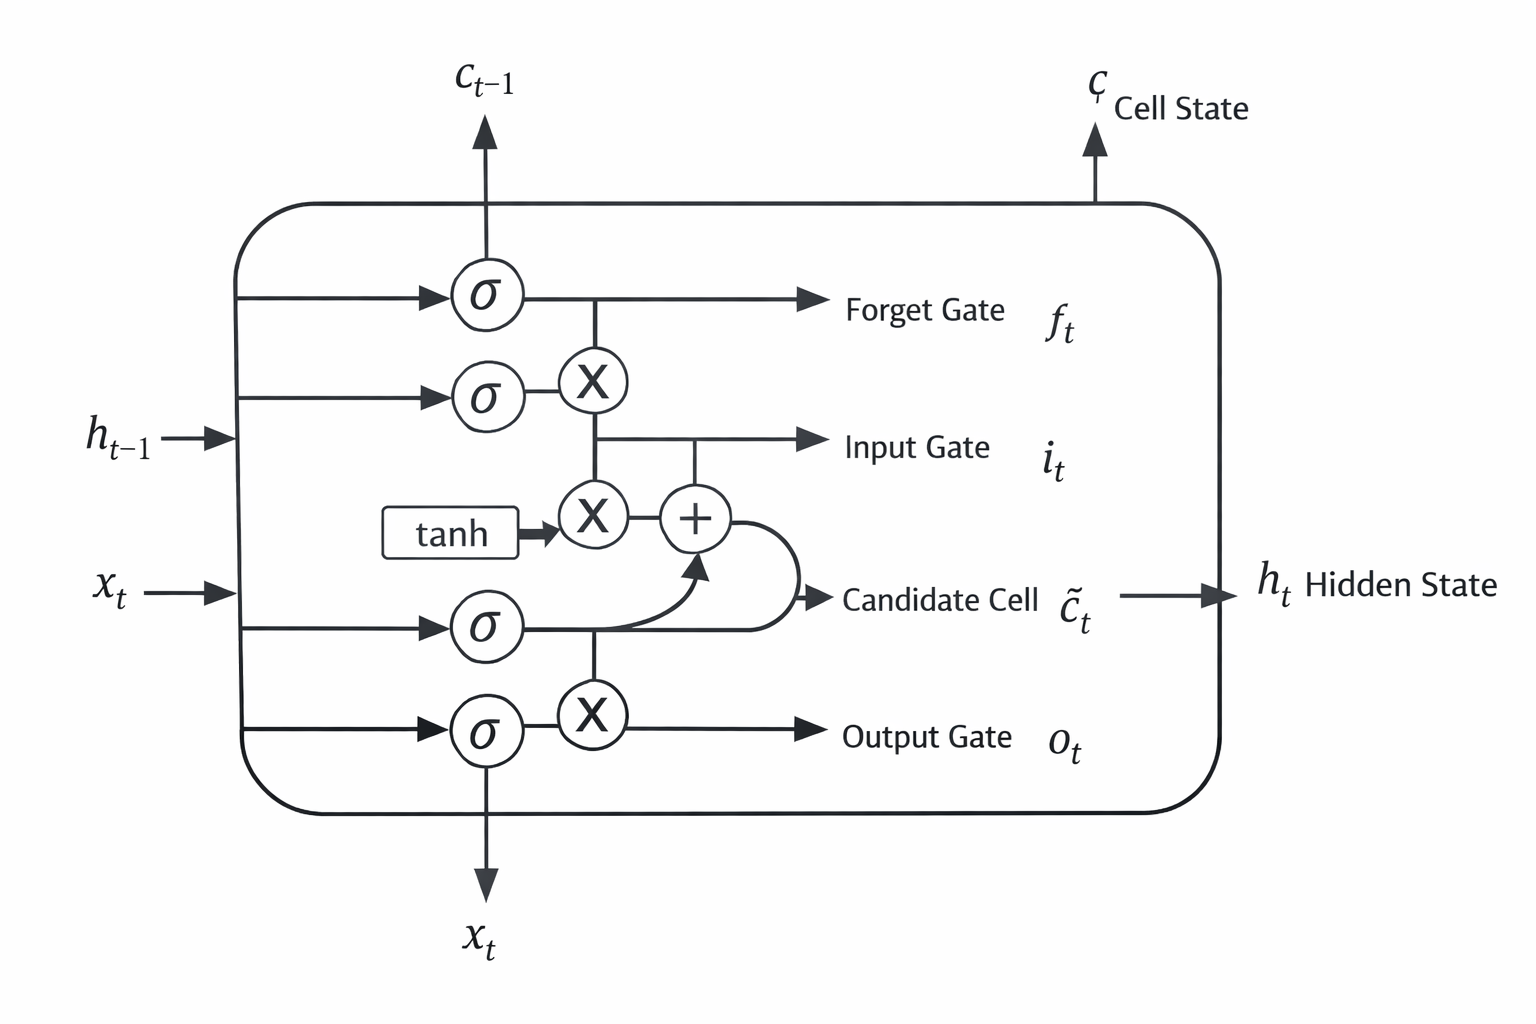
\includegraphics[width=0.9\textwidth]{picture/lstm.png}
\caption{Architecture of the LSTM network}
\end{figure}
\begin{equation}
i_t = \sigma \left( W^{(i)} X_t + U^{(i)} O_{t-1} \right),
\tag{4}
\end{equation}
\begin{equation}
f_t = \sigma \left( W^{(f)} X_t + U^{(f)} O_{t-1} \right),
\tag{5}
\end{equation}
\begin{equation}
\tilde{S}_t = \tanh \left( W^{(c)} X_t + U^{(c)} O_{t-1} \right),
\tag{6}
\end{equation}
\begin{equation}
S_t = f_t \circ S_{t-1} + i_t \circ \tilde{S}_t,
\tag{7}
\end{equation}
\begin{equation}
o_t = \sigma \left( W^{(o)} X_t + U^{(o)} O_{t-1} \right),
\tag{8}
\end{equation}
\begin{equation}
O_t = o_t \circ \tanh (S_t).
\tag{9}
\end{equation}

\subsection{Gated recurrent unit (GRU).}
Gated Recurrent Unit (GRU) is a type of recurrent neural network (RNN) that employs gating mechanisms to regulate the flow of information through hidden states \cite{Cho2014GRU,Sutskever2014Seq2Seq,Che2018GRUD}. Let $W_z$, $W_r$, $W$, $U_z$, $U_r$, $U$, $b_z$, $b_r$, and $b$ denote the model parameters, and let $\odot$ represent element-wise multiplication. For the $j$-th hidden unit, the GRU introduces a reset gate $r_t^j$ and an update gate $z_t^j$ to control the hidden state $h_t^j$ at each time step $t$. The mathematical formulation of the GRU unit is expressed in Eqs.~(10)--(13) as follows:
\begin{figure}[h]
\centering
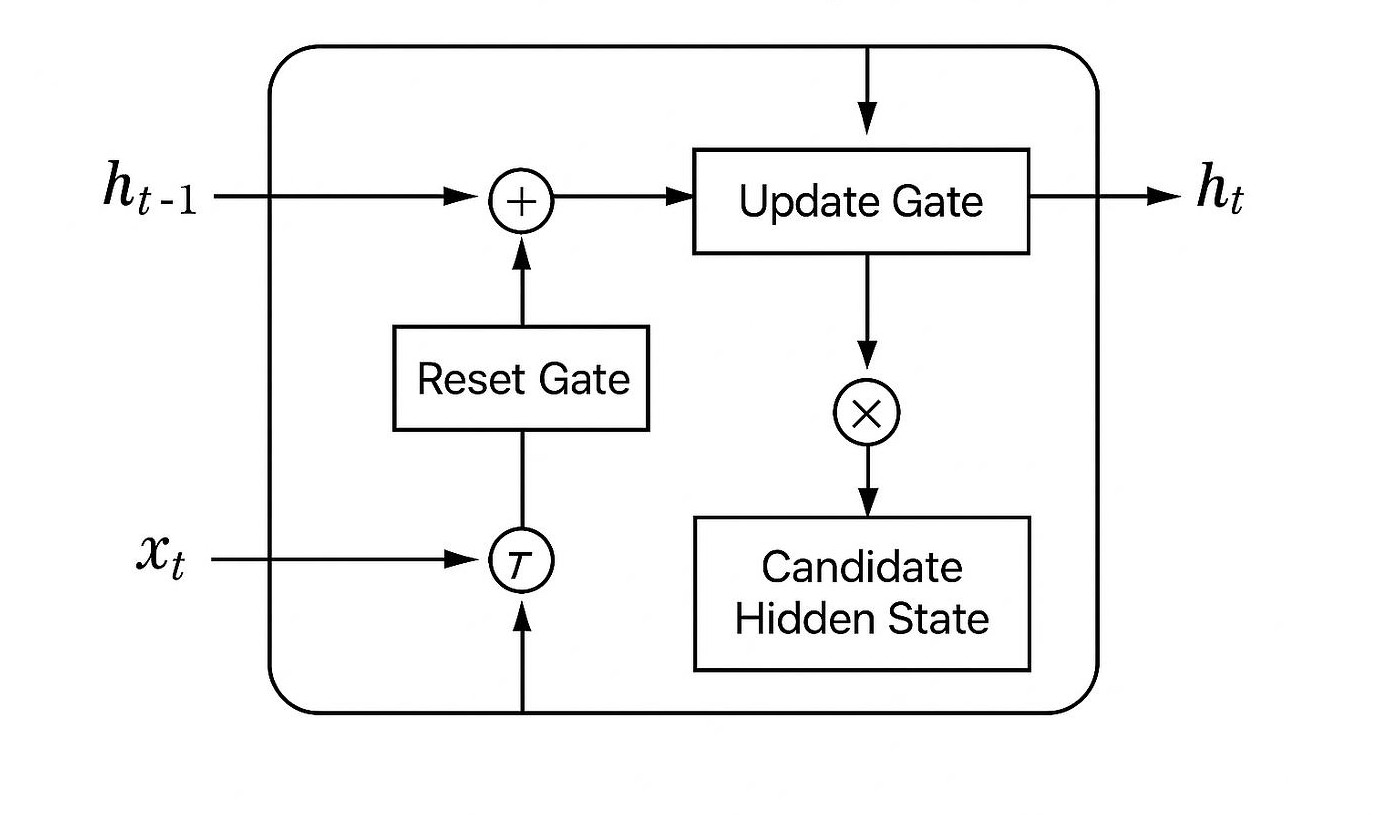
\includegraphics[width=0.9\textwidth]{picture/gru.jpeg}
\caption{Architecture of the GRU network}
\end{figure}
\begin{equation}
z_t = \sigma \left( W_z X_t + U_z h_{t-1} + b_z \right),
\tag{10}
\end{equation}
\begin{equation}
r_t = \sigma \left( W_r X_t + U_r h_{t-1} + b_r \right),
\tag{11}
\end{equation}
\begin{equation}
\tilde{h}_t = \tanh \left( W X_t + U \left( r_t \odot h_{t-1} \right) + b \right),
\tag{12}
\end{equation}
\begin{equation}
h_t = \left( 1 - z_t \right) \odot h_{t-1} + z_t \odot \tilde{h}_t .
\tag{13}
\end{equation}
\subsection{Evaluation metrics}
The criteria by which model performance is assessed must be clearly identified (ref.). In this research model performance is goind to be assessed on four statistical indexes.

\subsubsection{Coefficient of determination ($R^2$)}
R$^{2}$ is ratio of the disparity in the dependent variable which is predicted by the aid of independent variable. It is an indicator generated from regression analysis. In linear regression, the R$^{2}$ is also equal to the square of the correlation (R) between predicted P-value and actual O-values; owing to this, it is value from 0 to 1. In no correlation case, R$^{2}=0$ which means the independent variable incapable to predict the dependent variable. In no correlation error, R$^{2}=1$ which means the independent variable capable to predict dependent varibale with no error. If R$^{2}$ is between 0 and 1 refere to what extent is the ability of predicting the dependent variable.
\begin{equation}
R^2 = 1 - 
\frac{\sum_{i=1}^{n}(O_i - P_i)^2}
{\sum_{i=1}^{n}(O_i - O_m)^2},
\qquad 0 \leq R^2 \leq 1
\label{eq:r_square}
\end{equation}

\subsubsection{Mean square error (MSE)}
Mean Square Error (MSE) is an indicator for the predicting data by measuring the average of the squares of the errors in which obtained from the average squarred difference among the predicted data and observed data. Indeed, it describes how to set of points is near to the regression line. As shown in Eq.~\eqref{eq:meansquareerror}, it does this by taking the distances from the points to the regression line (these distance are the "error") and squaring them. Squaring is necessary to remove any negative signs.

\begin{equation}
\mathrm{MSE} = \frac{1}{n} \sum_{i=1}^{n} \left( y'_i - y_i \right)^2
\tag{15}
\label{eq:meansquareerror}
\end{equation}

\subsubsection{Root mean square error (RMSE)}
It is an ordinary approach to identify the model's error in predicting quantitative data.
\begin{equation}
\mathrm{RMSE} = \sqrt{ \frac{1}{n} \sum_{i=1}^{n} \left( y'_i - y_i \right)^2 }
\tag{16}
\label{eq:rootmeanse}
\end{equation}

\subsubsection{Mean Absolute Error (MAE)}
Mean Absolute Error (MAE) is a metric used to evaluate the accuracy of a predictive model by measuring the average magnitude of the absolute differences between predicted values and actual observed values. It indicates how far, on average, the predictions deviate from the true values, without considering the direction of the errors. A lower MAE value indicates better model performance.

%The evaluation metrics used for forecasting are the mean absolute error (MAE), mean square error (MSE), and root mean square error (RMSE). MAE reflects the actual magnitude of the prediction error, while RMSE evaluates the variability and accuracy of the data. Let $y'_i$, $y_i$, and $n$ denote the predicted value, the true value, and the number of samples, respectively. Equations (14--16) are used to calculate MAE, MSE, and RMSE, respectively 

\begin{equation}
\mathrm{MAE} = \frac{1}{n} \sum_{i=1}^{n} \left| y'_i - y_i \right|
\tag{14}
\end{equation}

\subsubsection{Uncertaintly Analysis}

\subsubsection{Model selection}
In this research, GRU and LSTM in terms of 24-and 12-hours datasets. The compariosn among all models will be implemented based on the performance indicator (R$^{2}$, RMSE, MSE, MAE, and WI). Furthermore, Taylor Diagram is constructed to clearly distinguish between all the prediction model utilized. Additionally, the uncertainty analysis is investigated for the best model selected, which is MLP, where the level of 95\% confidence and b-factor are identified.

\subsection{Dataset}
This paper use AQI and satellite data ERA5 conditions in Indonesia. The AQI data owned by DKI Jakarta Provincial Government can be accessed at (perlu cite aja). The air quality dataset is daily records Air Quality Index (AQI) of  PM$_{2.5}$, SO$_{2}$, CO, and NO$_{2}$ from 2014 to 2024.

%========================================================================================================================================

\section{Results}
\label{sec3}
The datasets are containing less than 5\% missing values. The missing values are filled up using an average value of the observed variables from 7 days before the observed date. After preprocessing phase, it implements column-based integration to create a single formed data from AQI and meteorological condition datasets. The integrated data is used to generate a causal graph and to train models for forecasting.

\subsection{Causality analysis}
This study investigates the causal dependency structure between air pollutants and meteorological conditions using the PC algorithm. The analysis was conducted on an integrated dataset covering the period from 2014 to 2024 7 variables: temperature, rainfall, BLH, PM$_{2.5}$, SO$_2$, CO, O$_3$, and NO$_2$.

\begin{figure}[htbp]
    \centering
    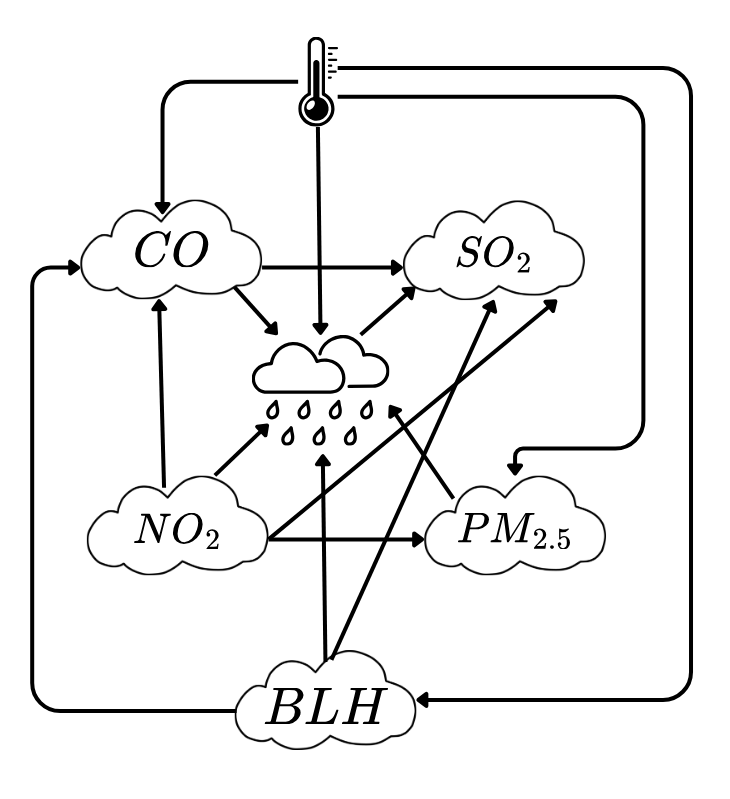
\includegraphics[width=0.5\linewidth]{./picture/grafik.png}
    \caption{Causal graph generated using the PC algorithm ($\alpha = 0.05$).}
    \label{fig:causal_graph}
\end{figure}

Figure~\ref{fig:causal_graph} illustrates the causal graphs generated using the PC algorithm ($\alpha = 0.05$). The graphs reveal direct and indirect relationships among meteorological variables and air pollutants.

\subsection{Correlation Analysis}

This study highlights Pearson correlation coefficients ($\rho$) with values satisfying $|\rho| \geq 0.2$. Figure~\ref{fig:heatmap} presents the correlation coefficients among temperature, precipitation, BLH, PM$_{2.5}$, CO, NO$_2$, and SO$_2$.

\begin{figure}[htbp]
    \centering
    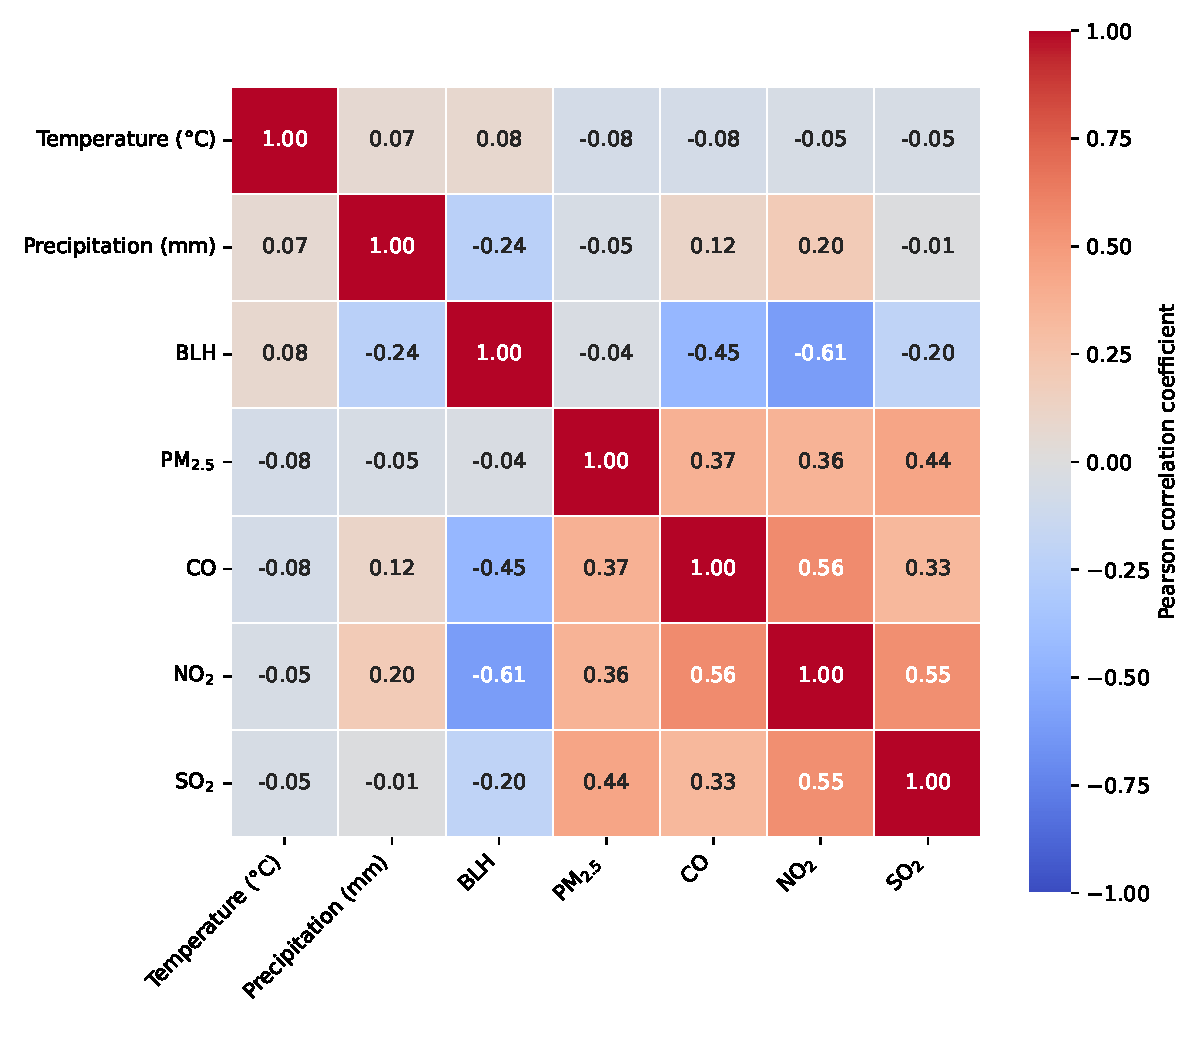
\includegraphics[width=0.7\linewidth]{./picture/correlation_heatmap.pdf}
    \caption{Pearson correlation heatmap between meteorological variables and air pollutants.}
    \label{fig:heatmap}
\end{figure}

BLH shows negative correlations with precipitation ($\rho=-0.24$), CO ($\rho=-0.45$), NO$_2$ ($\rho=-0.61$), and SO$_2$ ($\rho=-0.20$), indicating that higher atmospheric mixing tends to reduce pollutant concentrations. PM$_{2.5}$ is positively correlated with CO ($\rho=0.37$), NO$_2$ ($\rho=0.36$), and SO$_2$ ($\rho=0.44$), suggesting common emission sources and atmospheric processes. Strong positive correlations are also observed between CO and NO$_2$ ($\rho=0.56$) and between NO$_2$ and SO$_2$ ($\rho=0.55$). In contrast, temperature exhibits weak correlations with all other variables ($|\rho|<0.1$). Overall, the results highlight strong interactions among air pollutants and the important role of BLH in regulating air quality.

\subsection{Study Area}

This study was conducted over the Indonesian domain, covering the entire archipelago at a spatial resolution of 0.75°~$\times$~0.75° to align with the ERA5 grid configuration. Rather than focusing on a limited number of ground observation stations for model training, independent GRU and LSTM models were trained for each individual grid cell across the domain. This grid-based approach generates both daily and monthly predictions for PM\textsubscript{2.5}, CO, NO\textsubscript{2}, and SO\textsubscript{2} at every grid point, enabling full spatial coverage across Indonesia and capturing the high spatial heterogeneity of emission sources, land cover, and meteorological conditions that characterize the archipelago.

\begin{figure}[htbp]
    \centering
    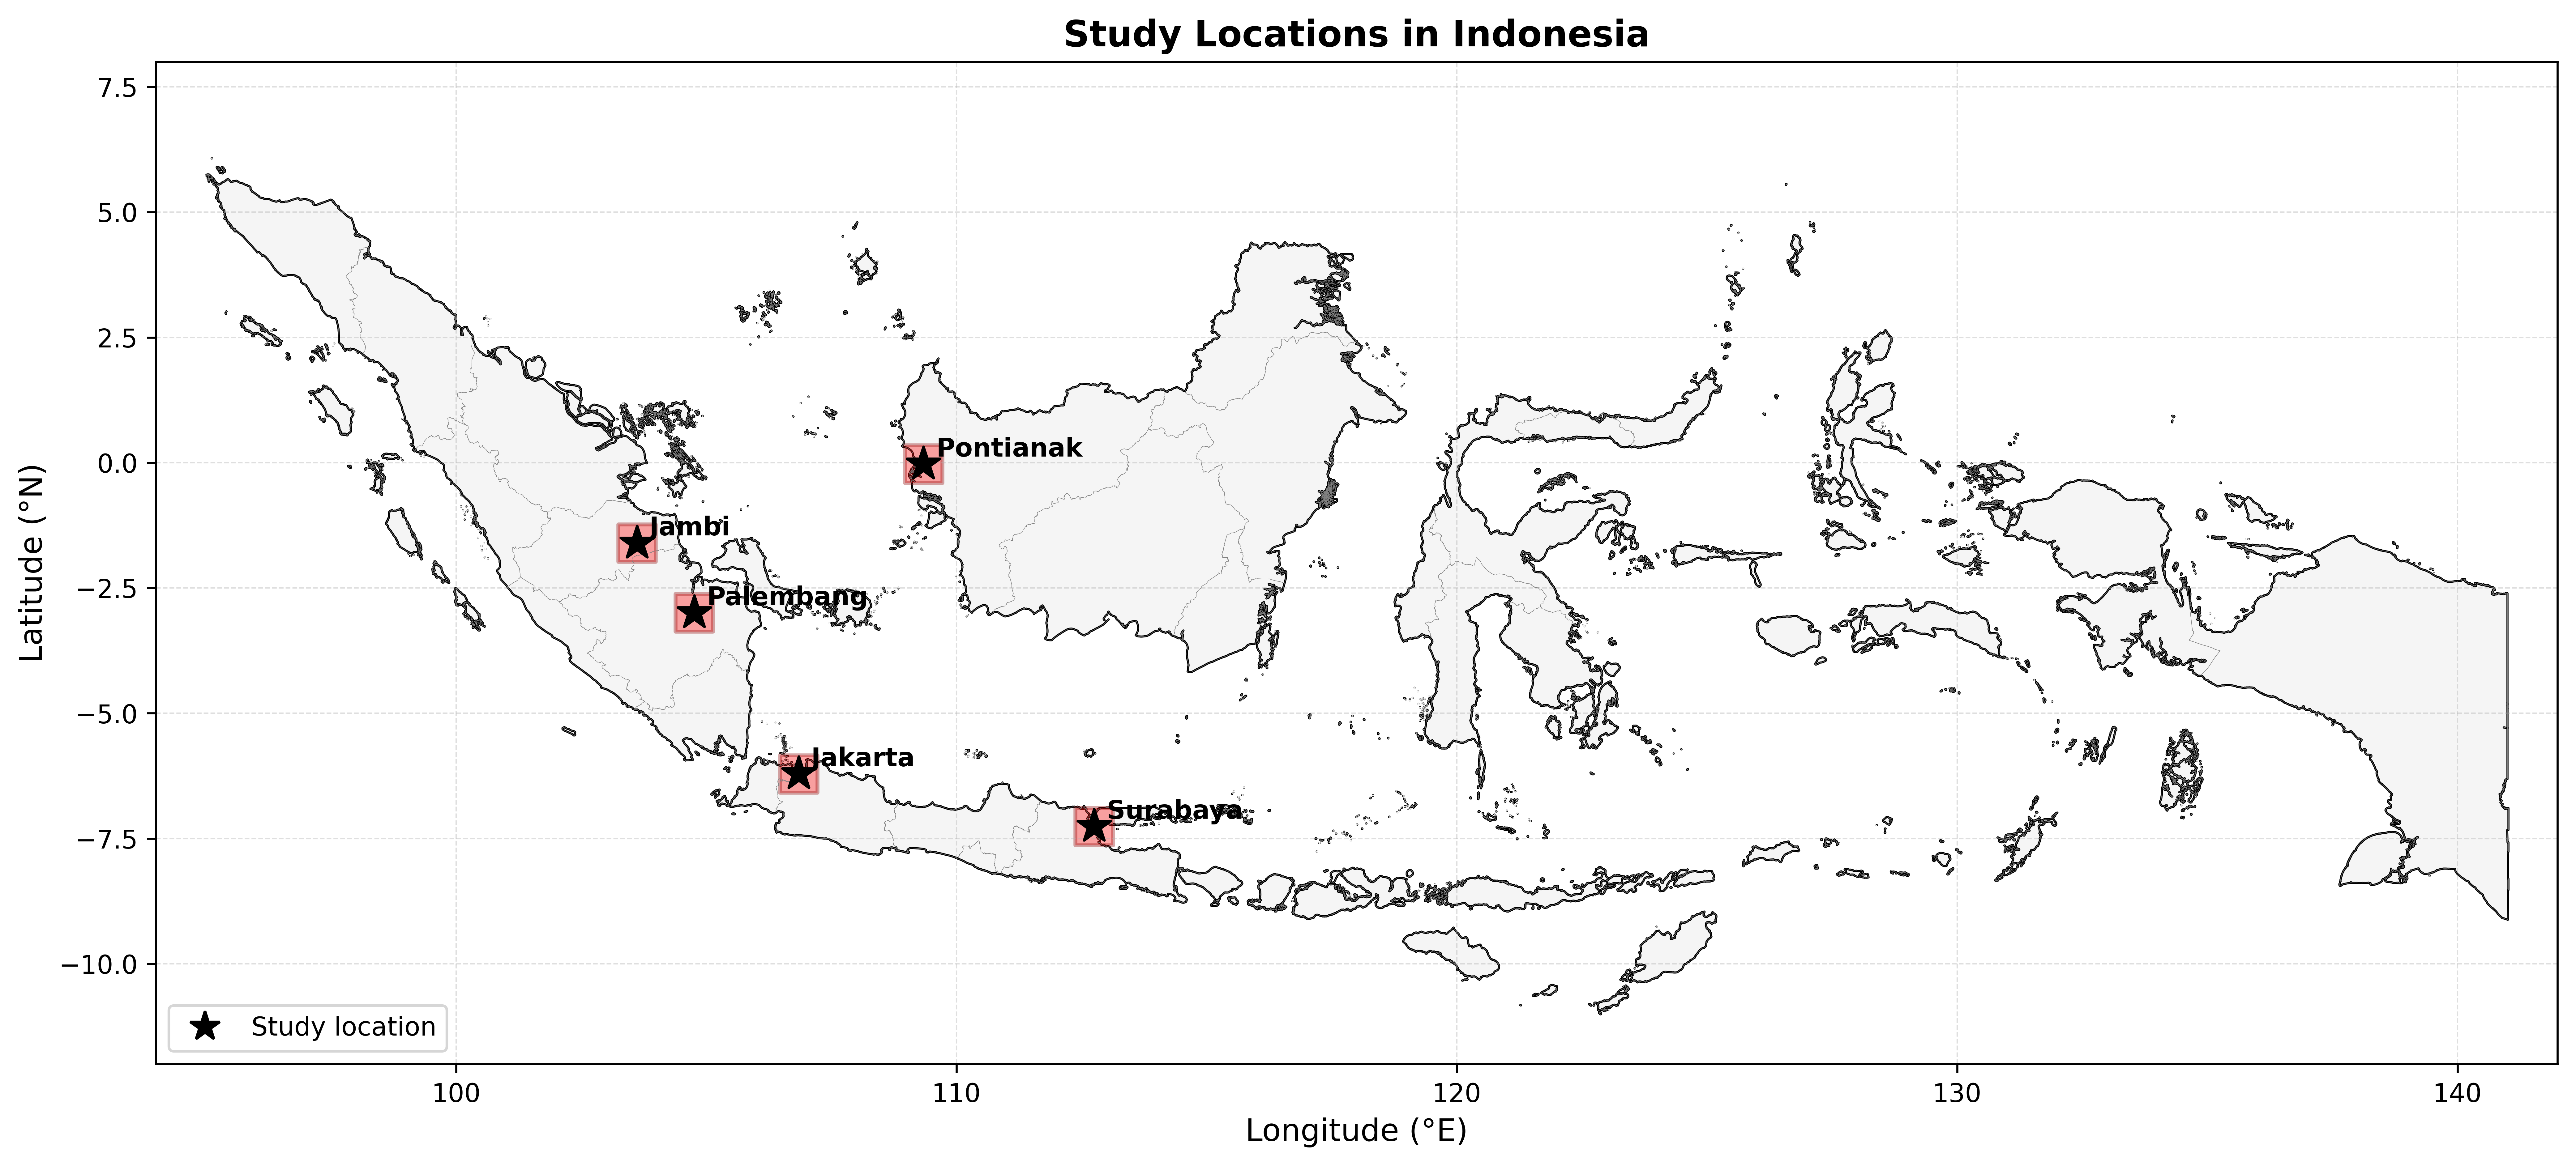
\includegraphics[width=0.9\linewidth]{./picture/peta.png}
    \caption{Geographical distribution of the five representative study locations across the Indonesian}
    \label{fig:heatmap}
\end{figure}

To validate the model predictions and evaluate their performance , five major cities were selected as benchmark reference stations to represent the country's diverse pollution regimes and geographic settings: Jakarta, Surabaya, Pontianak, Palembang, and Jambi (Figure~\ref{fig:map}). Specifically, Jakarta (6.21°S, 106.85°E) and Surabaya (7.25°S, 112.75°E) exemplify densely populated urban environments on Java Island, where air quality is predominantly driven by vehicular traffic and industrial emissions. Conversely, Pontianak (0.02°N, 109.34°E) in West Kalimantan, Palembang (2.99°S, 104.75°E) in South Sumatra, and Jambi (1.61°S, 103.61°E) in Jambi Province serve as representative cases for fire-prone regions, where seasonal peatland and forest burning cause episodic and severe air quality deterioration during the dry season.

By combining this spatially comprehensive grid-based modeling with localized validation, this framework provides a robust assessment of deep learning-based air quality forecasting across Indonesia, while ensuring high-fidelity quantitative evaluation at key hotspot locations.

\subsection{The historical data and forecasting models}

The observed data (OBS) reveal distinct spatiotemporal variability in air pollutant concentrations (PM\textsubscript{2.5}, CO, NO\textsubscript{2}, and SO\textsubscript{2}) across all stations during the 2021--2023 period. Notably, significant concentration spikes were recorded during mid-2022 to early 2023 in Pontianak, Palembang, and Jambi (panels C--H), which are consistent with the annual occurrence of peatland and forest fires in Kalimantan and Sumatra. These biomass burning episodes are well-documented drivers of episodic air pollution events in equatorial Indonesia, particularly elevating PM\textsubscript{2.5} and CO concentrations by several fold above baseline levels. In contrast, Surabaya (panels A--B) and Jakarta (panels I--J) exhibited relatively more stable concentration patterns throughout the study period, with pollutant levels primarily influenced by vehicular emissions and industrial activities rather than seasonal biomass burning.


Both the GRU and LSTM models demonstrated a reasonable capacity to capture the general temporal trends of the observed pollutant concentrations across all stations. In the full time-series panels (left panels: A, C, E, G, I), the predicted values from GRU and LSTM closely followed the OBS lines during periods of moderate pollution levels. However, during extreme episodic events --- particularly the pronounced peaks observed in Pontianak (panel C), Palembang (panel E), and Jambi (panel G) --- both models showed a tendency to underestimate peak concentrations, suggesting that the models may have difficulty capturing abrupt, short-duration pollution spikes driven by localized fire events. This limitation is common in deep learning-based forecasting models when training data contains imbalanced distributions of extreme values.

The monthly-averaged trend panels (right panels: B, D, F, H, J) provide a clearer picture of the seasonal forecasting performance. In Surabaya (panel B) and Jakarta (panel J), where seasonal fluctuations were more gradual, both GRU and LSTM produced smooth predictions that closely aligned with the observed monthly means across all four pollutants, indicating robust model generalization for stations with relatively homogeneous emission sources. For Pontianak (panel D), Palembang (panel F), and Jambi (panel H), the monthly-averaged predictions partially captured the seasonal pollution peaks, though the magnitude of peak-season concentrations was still slightly underestimated by both models, particularly for SO\textsubscript{2} and NO\textsubscript{2}.

\begin{figure}[htbp]
    \centering
    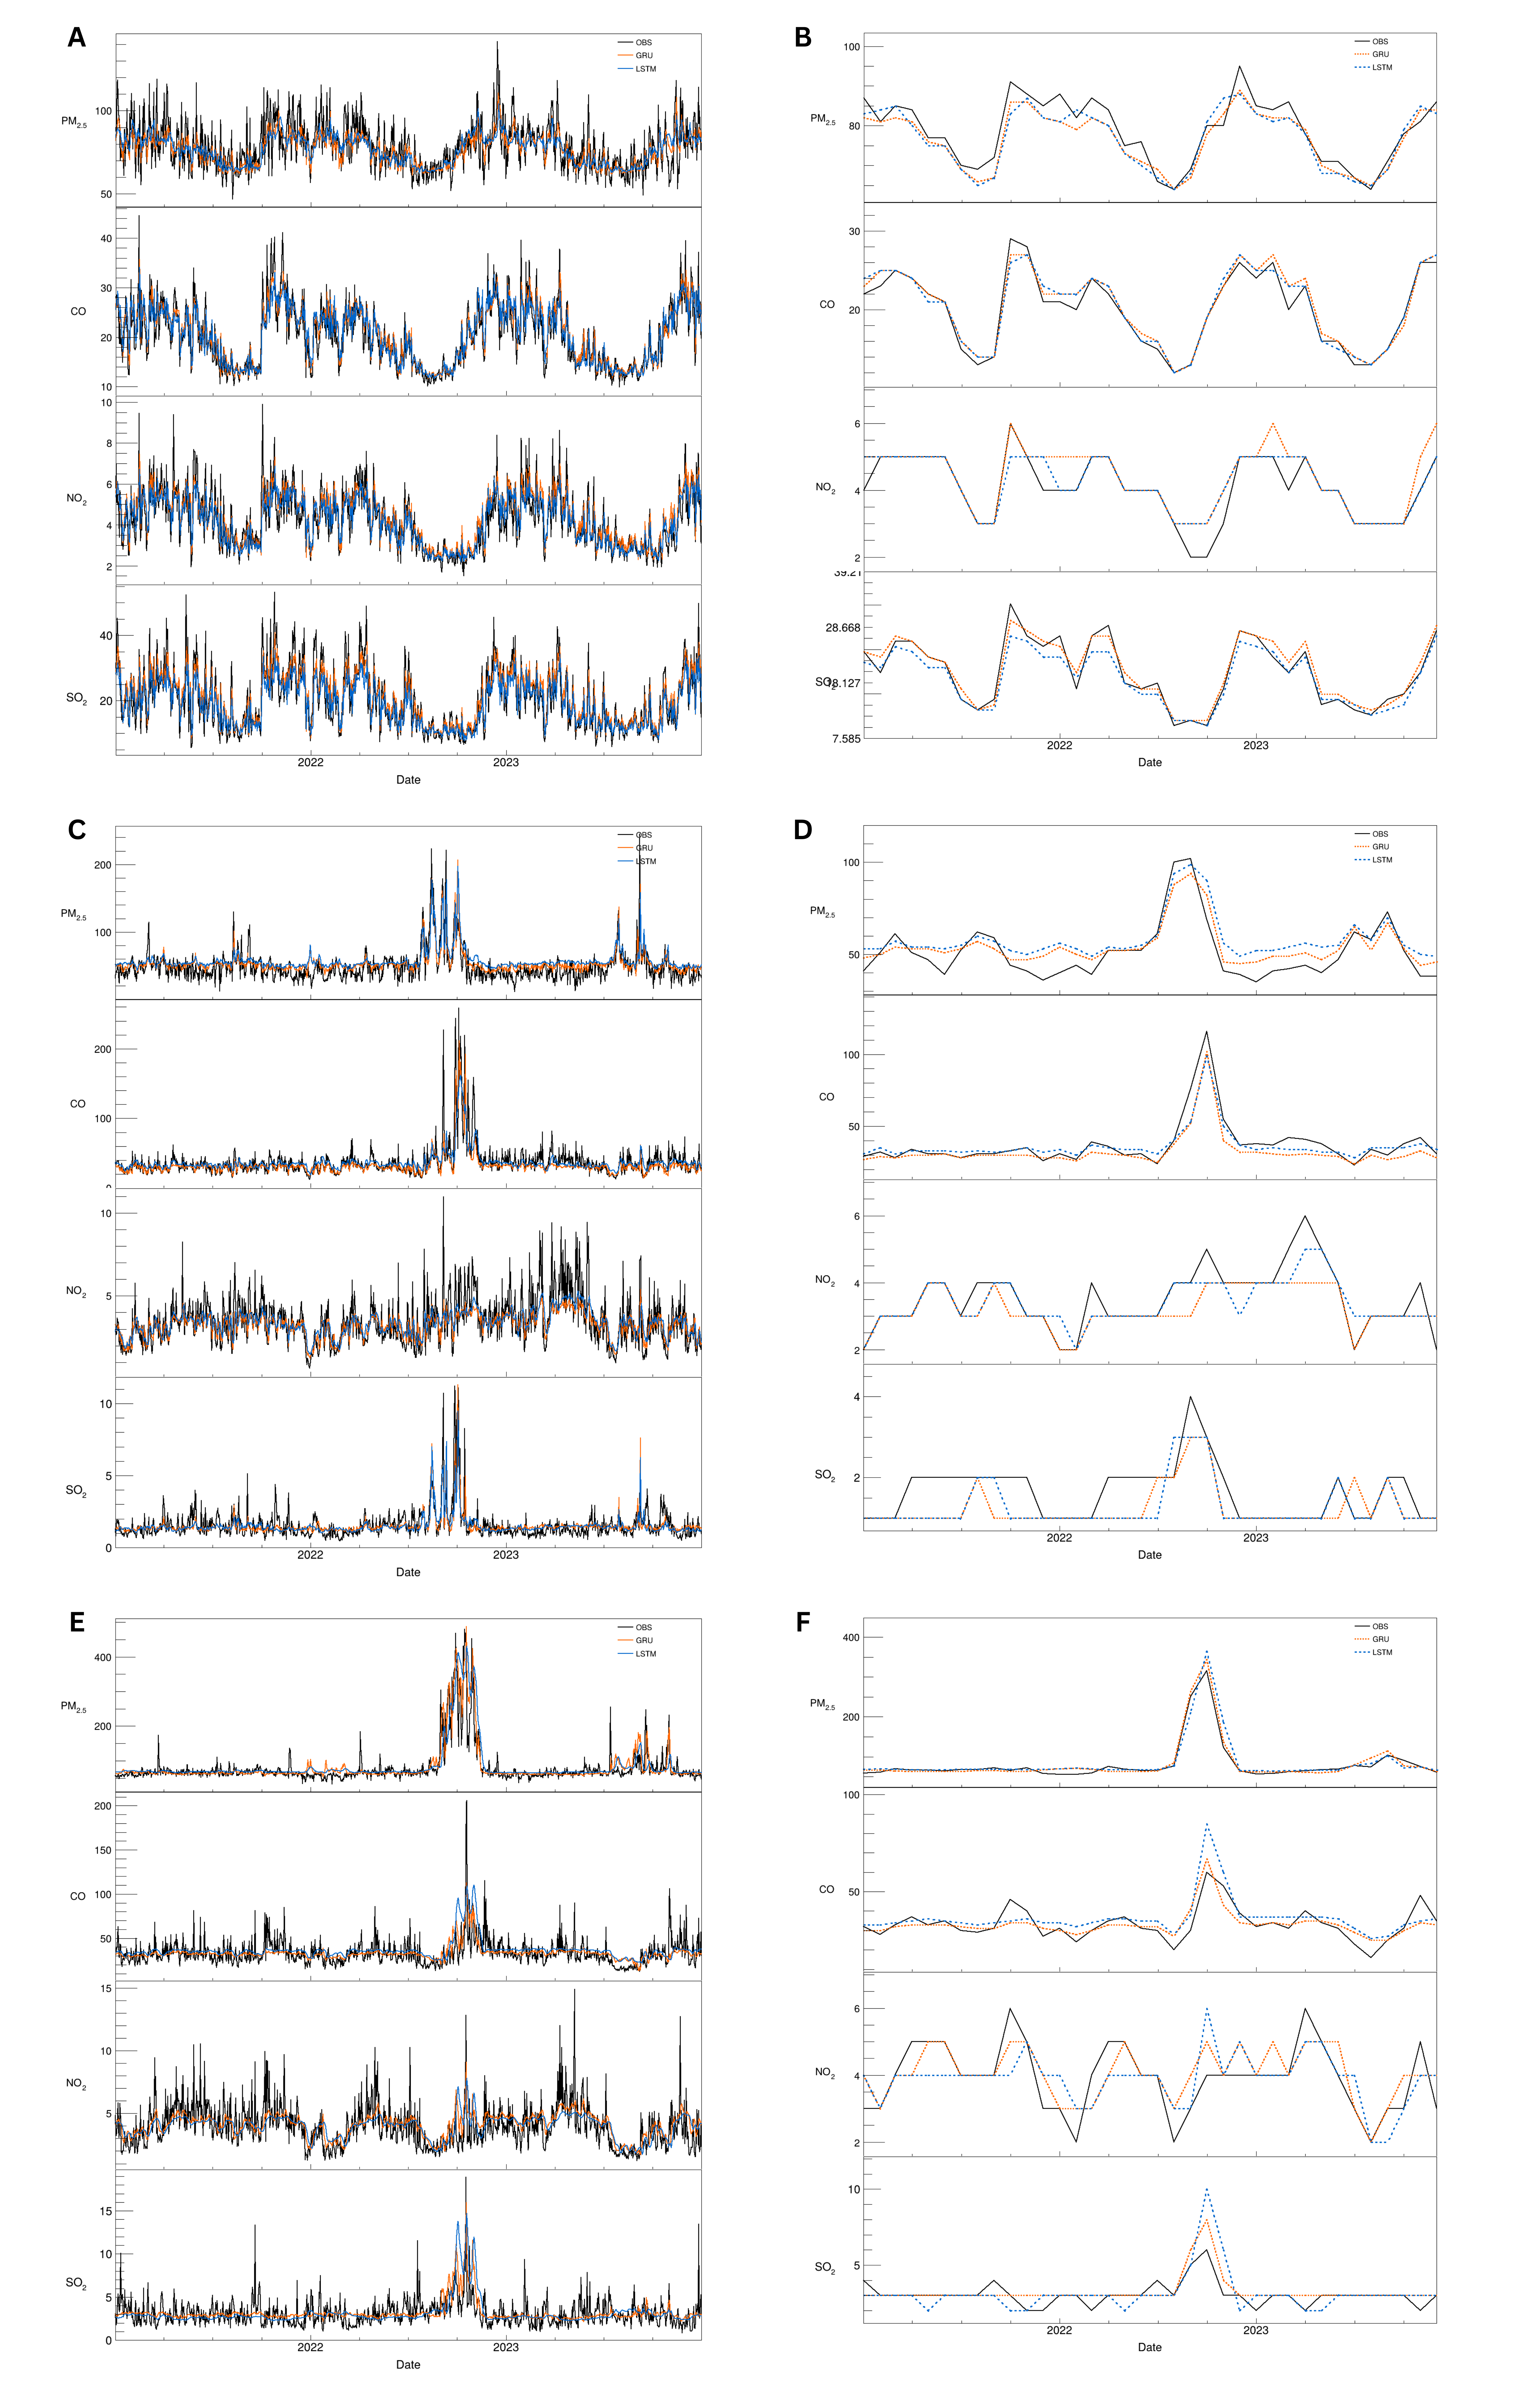
\includegraphics[width=1\linewidth]{./picture/grafik/1.png}
    \label{fig:heatmap}
\end{figure}

\begin{figure}[htbp]
    \centering
    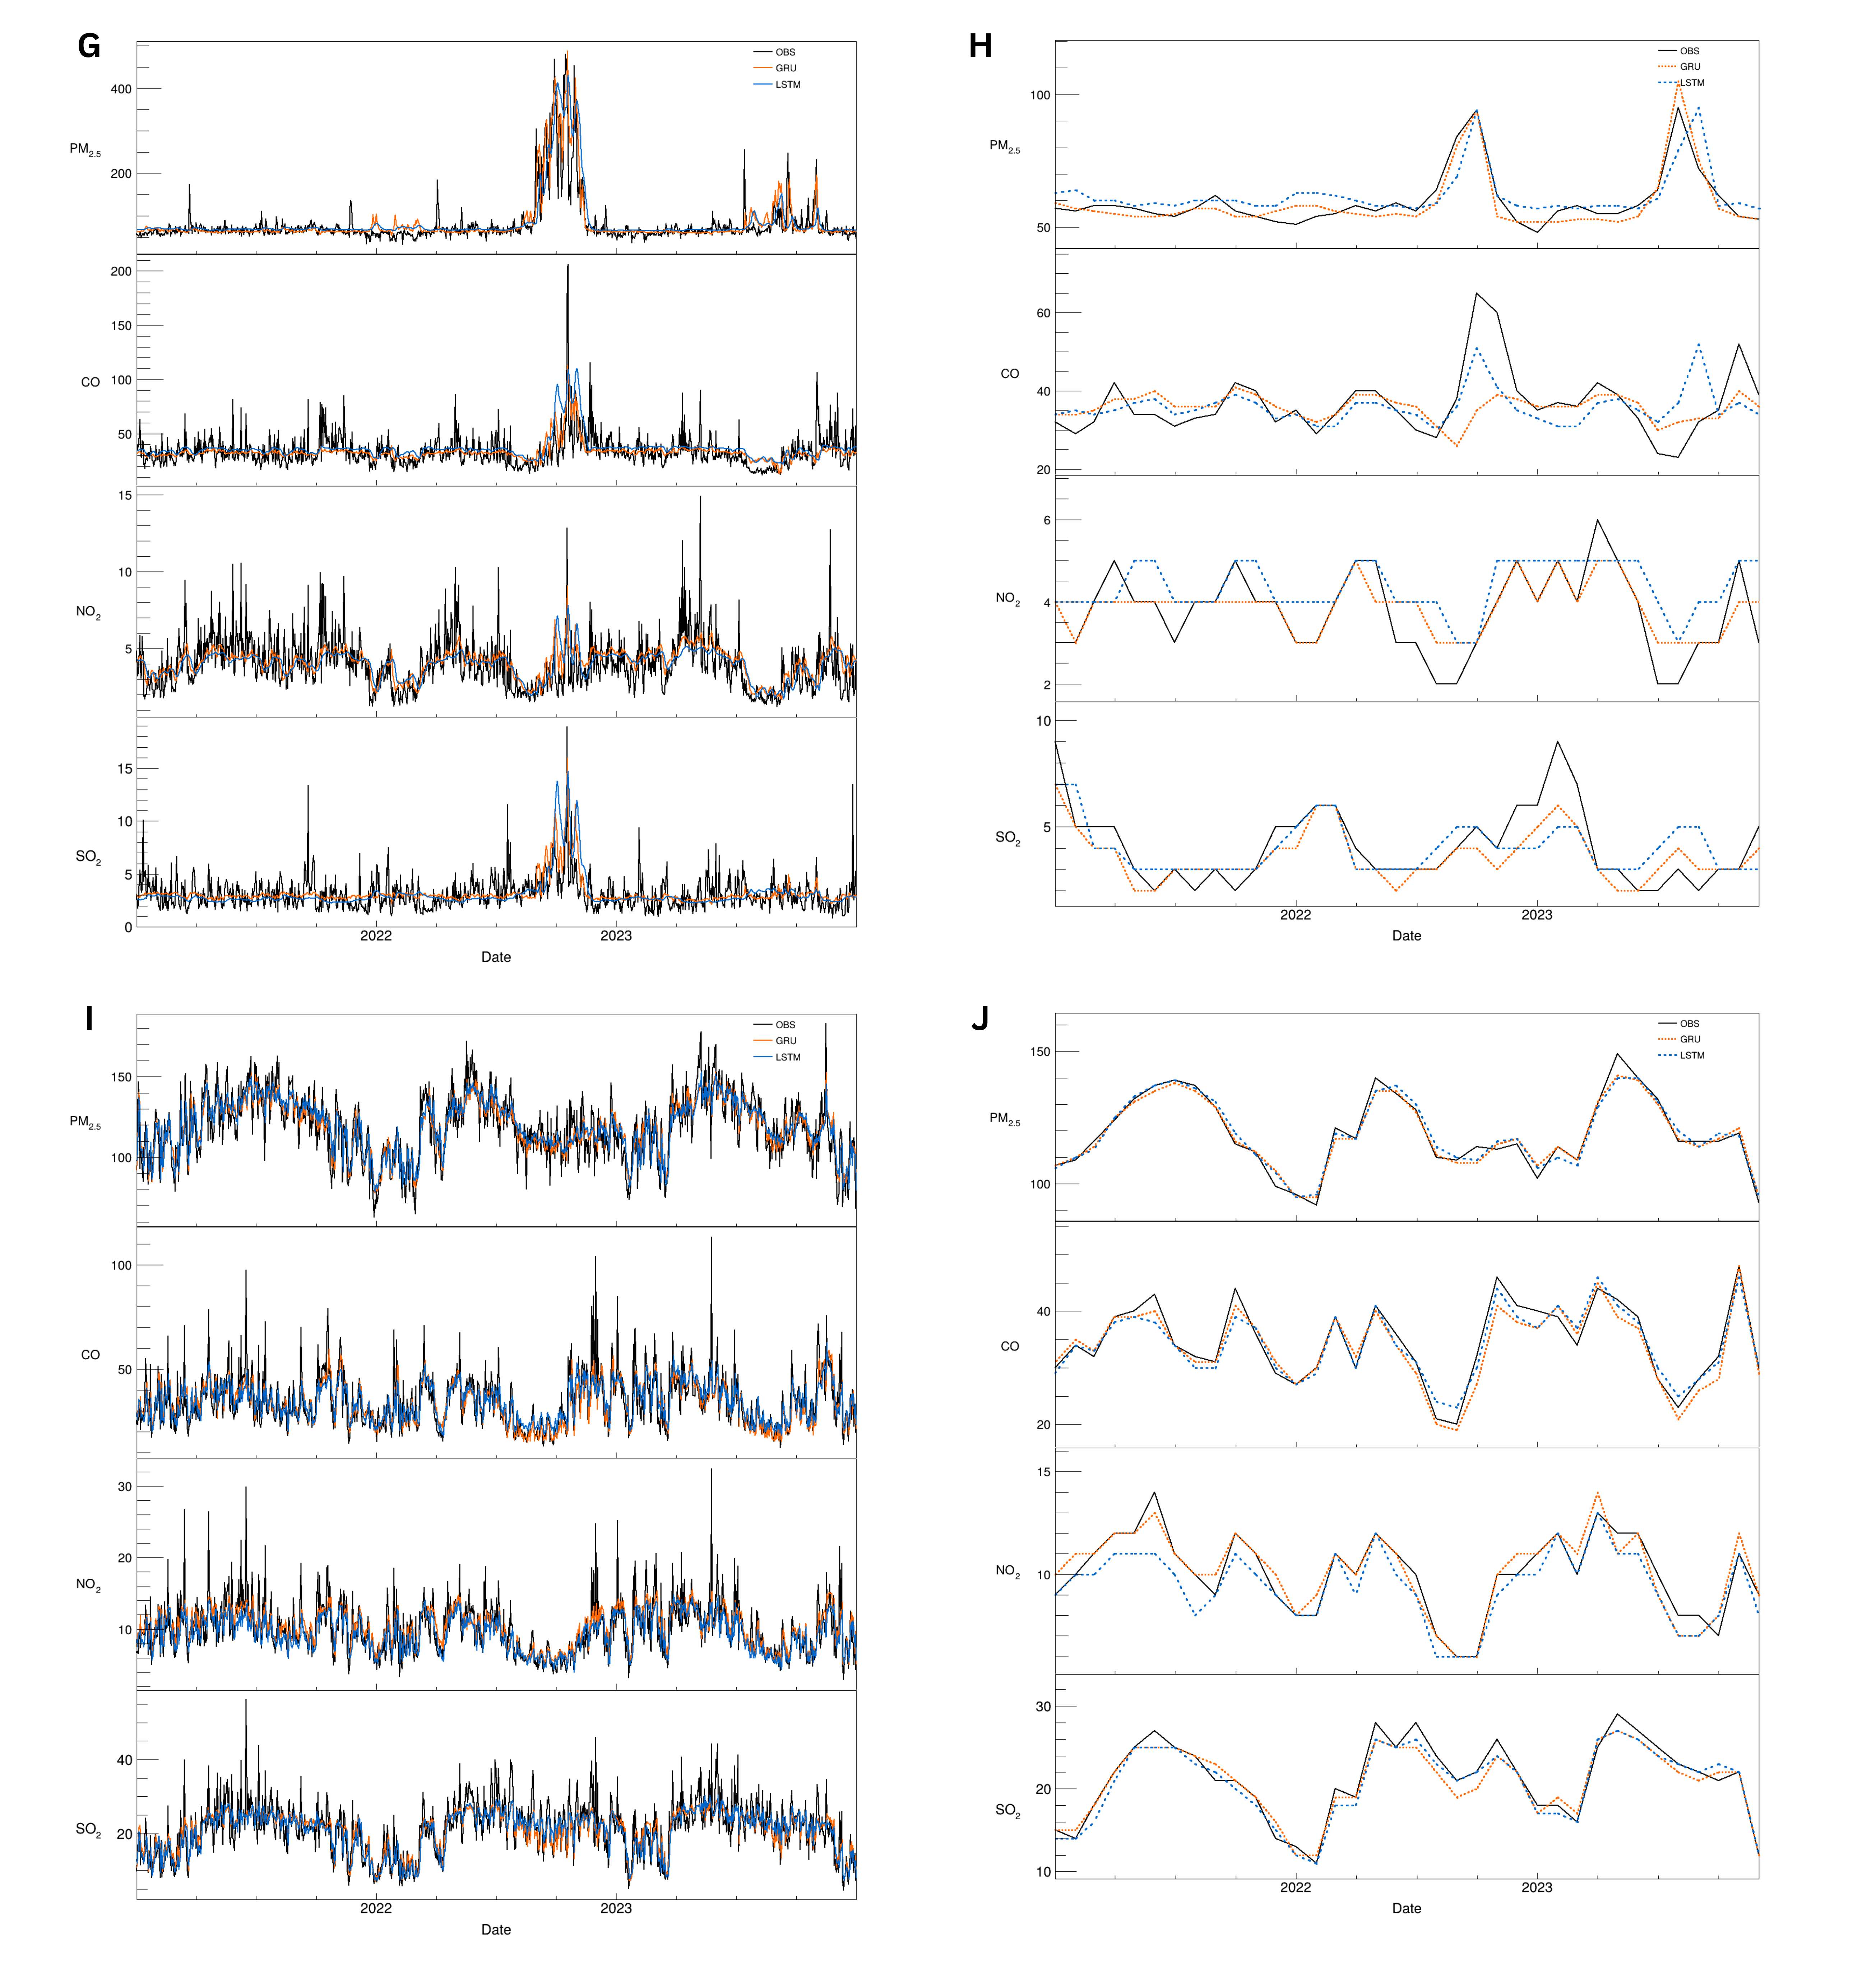
\includegraphics[width=1\linewidth]{./picture/grafik/2.png}
    \label{fig:heatmap}
\end{figure}

\begin{figure}[htbp]
    \centering
    \includegraphics[width=0.9\linewidth]{./picture/eval.png}
    \caption{Boxplot distributions of forecasting performance metrics (MAE, RMSE, and $R^2$).}
    \label{fig:boxplot_metrics}
\end{figure}


Comparing the two architectures, the GRU model generally exhibited slightly tighter agreement with observed values during normal pollution episodes, while the LSTM model showed marginally better performance in tracking the recovery phase following peak pollution events. This is consistent with the architectural difference between the two models: LSTM's more complex gating mechanism, comprising both forget and input gates, may confer a slight advantage in retaining long-term temporal dependencies, particularly useful for capturing the gradual decline in pollutant concentrations after extreme events. Meanwhile, the GRU's simplified architecture allows for faster convergence and may be less prone to overfitting on shorter training sequences. Nevertheless, the performance differences between GRU and LSTM were relatively small across all stations, suggesting that both architectures are comparably suited for air quality forecasting in the Indonesian urban context.


Figure~\ref{fig:boxplot_metrics} illustrates the distributions of MAE, RMSE, and $R^2$ obtained from GRU and LSTM models for PM$_{2.5}$, CO, NO$_2$, and SO$_2$ at daily and monthly forecasting scales. The results indicate that monthly forecasts consistently achieve lower MAE and RMSE values and higher $R^2$ scores compared with daily forecasts, demonstrating the benefit of temporal aggregation in reducing short-term variability and enhancing predictive performance. PM$_{2.5}$ and CO exhibit the largest prediction errors among the investigated pollutants, while NO$_2$ and SO$_2$ show substantially lower error distributions. Furthermore, monthly forecasts of NO$_2$ and SO$_2$ yield the highest predictive skill, with median $R^2$ values approaching or exceeding 0.8. The differences between GRU and LSTM are generally modest; however, GRU tends to provide slightly lower error metrics and marginally higher $R^2$ values in several cases, particularly for monthly predictions. These findings suggest that both deep learning architectures are effective for air-quality forecasting, while monthly aggregation leads to more robust and accurate predictions than daily forecasting.


%% The Appendices part is started with the command \appendix;
%% appendix sections are then done as normal sections
\appendix
\section{Example Appendix Section}
\label{app1}

Appendix text.

%% For citations use: 
%%       \cite{<label>} ==> [1]

%%

%% If you have bib database file and want bibtex to generate the
%% bibitems, please use
%%
%%  \bibliographystyle{elsarticle-num} 
%%  \bibliography{<your bibdatabase>}

%% else use the following coding to input the bibitems directly in the
%% TeX file.

%% Refer following link for more details about bibliography and citations.
%% https://en.wikibooks.org/wiki/LaTeX/Bibliography_Management

\bibliographystyle{elsarticle-num-names}
\bibliography{atmospheric.bib}

\end{document}
